\capitulo{5}{Aspectos relevantes del desarrollo del proyecto}

Lo más relevante de este proyecto es el transformar la última versión de Thoth a una aplicación web hecha por medio de GWT lo que supone comprender el funcionamiento interno del Thoth original, <<desmigajando>> para poder adaptarlo a las condiciones de un proyecto hecho con GWT.
Estas condiciones limitan un poco la aplicación y nos obligan a reformar partes que antes eran más sencillas.

Es el caso, por ejemplo del núcleo de la gramática de Thoth que no puede ser llevado a un proyecto en GWT tal cual y necesita ser adaptado para que funcione como en la aplicación original.
 
\section{Parser JavaCC}
GWT esta compuesto por una parte cliente que es la que será traducida a JavaScript y otra servidor escrita en Java. Lo ideal en una aplicación de este estilo sería incluir todo en el lado del cliente y olvidarse del resto, traduciendo todo a JavaScript para una ejecución fluida en la web. El caso es, que como no es fácil traducir de un lenguaje a otro, hay partes del Thoth antiguo que no pueden ir en el lado del cliente y por consiguiente traducirse a dicho lenguaje. Una de estas partes es el parser JavaCC.

Originalmente en el núcleo de Thoth dentro del directorio <<grammar>> colgaba un sub-directorio llamado <<parserjavacc>> en el cual se encontraba el parser para la gramática. Es la parte más importante dentro de la gramática ya que permite reconocer si esta está bien construida o no.
Ahora no procede explicar que es, pero si en que ha cambiado esta versión con respecto a la anterior. 
Para poder incluir esa parte en el proyecto decidimos hacerlo en el lado del servidor, ya que al no hacerse la traducción no habría ningún problema. Ahora bien lo más complicado de todo esto es la comunicación entre esas dos partes.
 
\subsection{Comunicación cliente-servidor}
Una vez alojado en el servidor el parser habrá que establecer una comunicación entre la parte del ciente en la que habrá un método que llame a la funcionalidad que se desee del servidor.

Para hacerlo, GWT utiliza la técnica denominada por sus siglas en inglés RPC o llamada de procedimiento remoto (Remote Procedure Call) que tiene una estructura similar a esta: 

\begin{figure}[h]
\centering
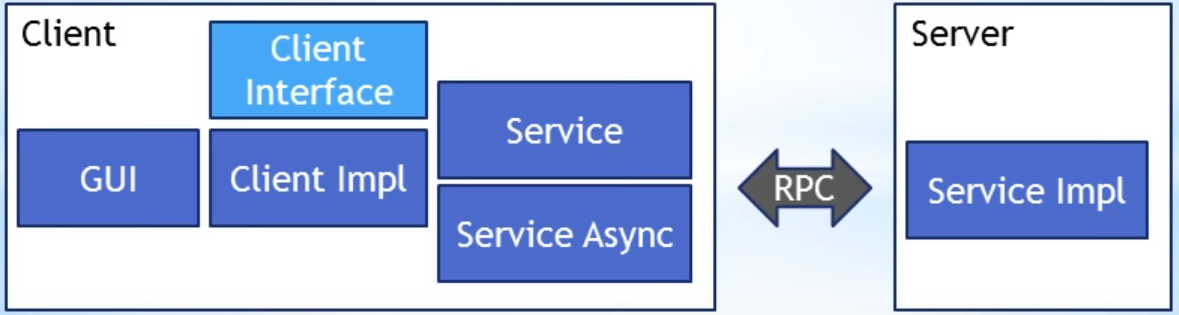
\includegraphics[width=0.65\textwidth]{RPC}
\caption{Arquitectura RPC simple.}
\label{fig:5.1}
\end{figure}

Del lado del cliente tenemos, en este caso, una interfaz gráfica de usuario (GUI), una clase dedicada a hacer las llamadas RPC (ClienImpl), dos interfaces que definen los métodos (Service y ServiceAsync), una clase con los métodos en el lado del servidor (serviceImpl) y por último una interfaz, que no es esencialmente necesaria (ClientInterface). 

En términos generales, para utilizar el parser de la gramática, que es quizá la clave de todo, hay que llamar al servidor y establecer una comunicación. Es ahí donde utilizamos la clase <<GrmmarServiceClientImp>> que hace las llamadas a las interfaces necesarias hasta llegar al servidor. Esta clase es un nexo de unión entre la parte del núcleo, que ese encuentra en el servidor y la parte del cliente que contiene lo visual y las acciones de los botones entre otros. La comunicación queda representada en este diagrama.

\begin{figure}[h]
\centering
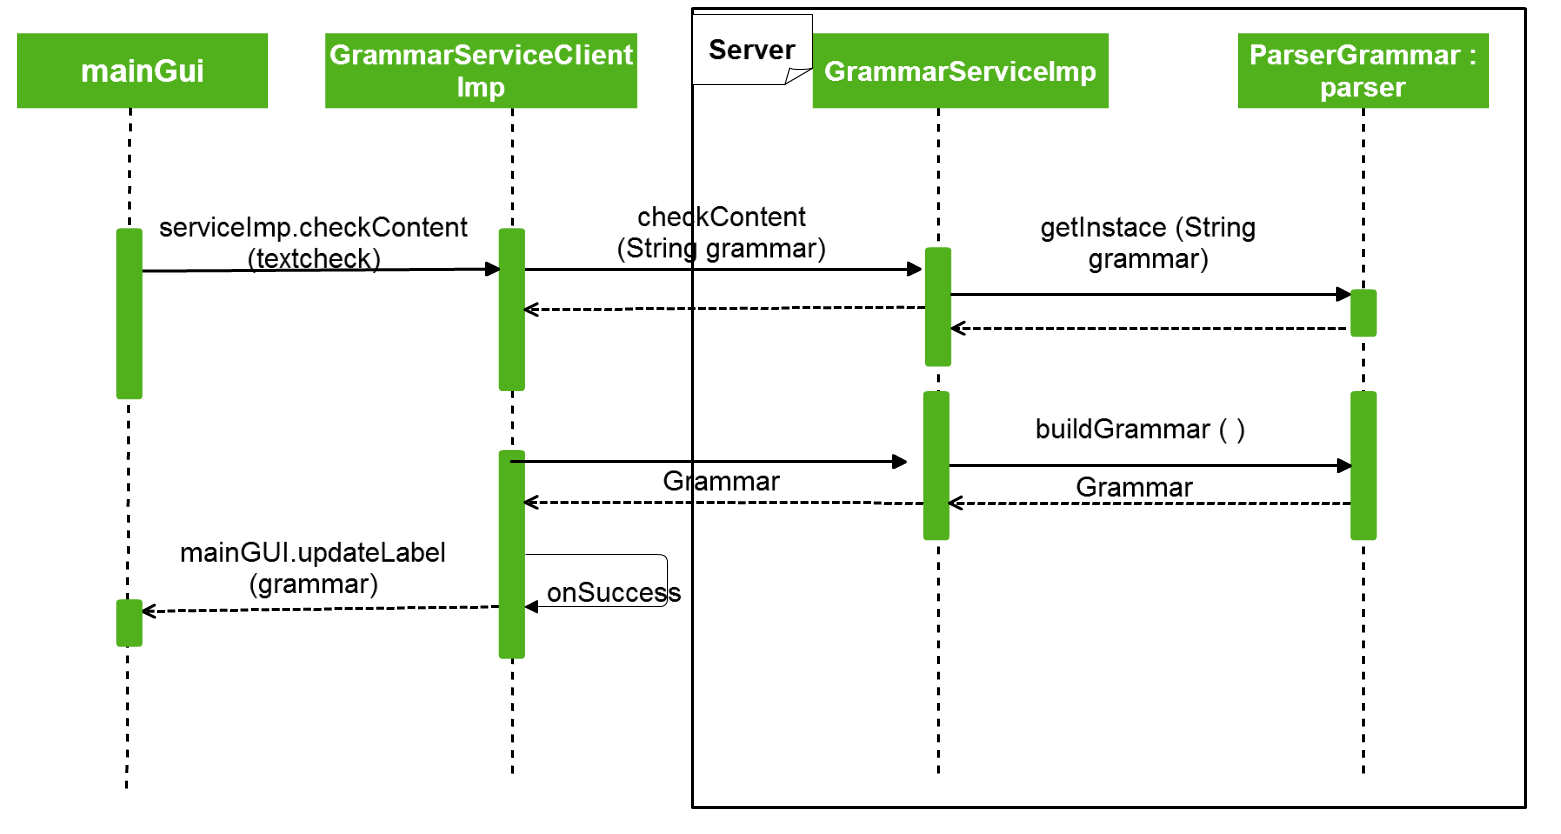
\includegraphics[width=0.65\textwidth]{ParserDiagram}
\caption{Diagrama sobre la comunicación entre el cliente y el servidor.}
\label{fig:5.1}
\end{figure}

Dentro de la clase <<GrammarServiceClientImp>> he creado dos constructores, uno al que le paso una url y otro una url y además una gramática para que construya, valga la redundancia, una nueva interfaz gráfica de usuario con dicha gramática. La url es simplemente la localización del <<servlet>> para la comunicación.

\section{Algoritmos}


\section{Internacionalización}
La aplicación cuenta con la funcionalidad de la internacionalización. Dentro del menú se pueden elegir entre varios idiomas a los que se traducirán los diferentes elementos. Los idiomas en los que está disponible la versión web de Thoth son: Alemán, castellano o español, francés y por supuesto inglés. Consideramos que esta funcionalidad es muy importante para poder llegar a diferentes países en el caso de que fuera necesario.

La internacionalización de la aplicación es un poco diferente a la utilizada en la versión de escritorio de Thoth. En primer lugar es necesario incluir una interfaz con los métodos para la internacionalización y los mensajes <<por defecto>> asociados a cada uno. Cada vez que queramos hacer uso de esos mensajes hay que hacer una llamada al método de la interfaz. Esa interfaz se encuentra en el directorio <<client.gui.utils>> donde se encuentran también los ficheros <<properties>> asociados, donde se encuentran las diferentes traducciones según el mensaje. Estos mensajes son los mismos que los utilizados para la internacionalización de Thoth V2.

Para poder realizar el cambio de idioma es necesario hacer uso de las propiedades las clases <<xml>> y <<html>> de GWT, en concreto <<locale>> que es la que especificará la localidad, que determina el idioma. Por ello cada vez que elegimos un idioma, la aplicación se redirige a una nueva <<URL>> (llevando a cabo una nueva compilación) con el atributo <<locale=>> seguido de las siglas del idioma al que se quiere traducir.